\subsection{The check with an incomplete or corrupt reference}\label{s:monitoring}

\begin{figure}[t]
  \centering
  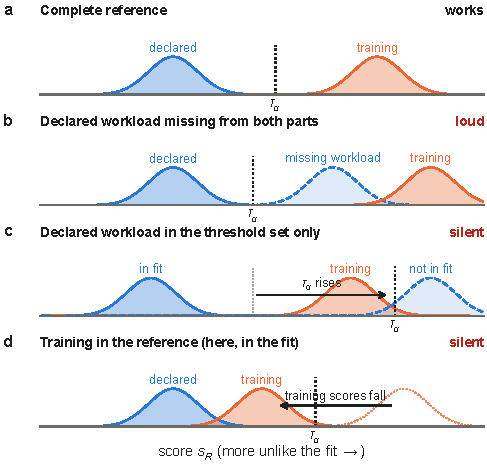
\includegraphics[width=\columnwidth]{f10_reference.pdf}
  \caption{The complete reference (a) and the three changes to it (b--d). Each curve is the distribution of
    the score $s_R$ for one kind of work: declared work (blue) or hidden training
    (orange). The monitor flags every window to the right of the threshold $\tau_\alpha$
    (dotted). (a) The fit and the threshold set hold every declared workload. Training is
    flagged, and declared work is not. (b) One declared workload (dashed) is in neither. It
    scores high and is flagged: a loud failure. (c) The same workload is in the threshold set
    but not in the fit. It still scores high, so $\tau_\alpha$ rises to meet it and
    passes training. Training is no longer flagged: a silent failure. Training in the
    threshold set acts the same way. (d) Training is in the fit. Its scores fall below
    $\tau_\alpha$, so the monitor misses it: also a silent failure. \Cref{t:t7,f:f9} hold the measured cases.}
  \label{f:f10}
\end{figure}

\begin{table*}[tp]
  \centering
  \small
  \resizebox{\textwidth}{!}{% generated by scripts/table_t7.py from (repo_commit of each source):
% h2 41b1fed, r1_scores 53f9463, episodes c574166, false_alarms 1fbe999, heldout dcd87a8, t4 1658809, manifest 018c3a2
% cell sources:
%   full: fit r1_scores.fit_runs.r1; tau set r1_scores.calibration_runs; co-location h2.headline.Z_r1.detection; episodes episodes.detectors.r1.counts; onsets false_alarms.backgrounds.{declared inference,idle}.r1.onsets
%   prefill held out: fit heldout.fit_runs minus panel-serving-prefill; tau set heldout.calibration_runs; flagged heldout.results[family=iforest,variant=R1,alpha=0.05].check4.per_run.panel-serving-prefill.fp_rate; co-location, episodes, onsets: none
%   decode only, decode: fit t4.misspecified_declaration.fit_runs; tau set t4.misspecified_declaration.calibration_runs.declared; co-location t4.misspecified_declaration.declared.h2.r1.co-location.pooled; episodes t4.misspecified_declaration.declared.h3.r1.episodes.counts; flagged t4.misspecified_declaration.declared.dev_stress_fpr; onsets t4.misspecified_declaration.declared.h3.r1.false_alarms.{declared inference,idle}.onsets
%   decode only, decode + idle: fit t4.misspecified_declaration.fit_runs; tau set t4.misspecified_declaration.calibration_runs.pooled; co-location t4.misspecified_declaration.pooled.h2.r1.co-location.pooled; episodes t4.misspecified_declaration.pooled.h3.r1.episodes.counts; flagged t4.misspecified_declaration.pooled.dev_stress_fpr; onsets t4.misspecified_declaration.pooled.h3.r1.false_alarms.{declared inference,idle}.onsets
\begin{tabular}{lllrrlrl}
\toprule
reference & unlike the fit & in $\tau$ set & co-location (\%) & episodes & unlike-fit work flagged (\%) & onsets dec.\ / idle & failure \\
\midrule
complete reference & -- & -- & 100.0 & 0 of 188 missed & -- & 0 / 1 & none \\
prefill held out of the fit & prefill & none & -- & -- & prefill 100.0 & -- & loud \\
decode-only fit, decode threshold set & prefill, idle & none & 100.0 & 164 of 188 start in alarm & prefill 100.0, idle 100.0 & 2 / 4 & loud \\
decode-only fit, decode + idle threshold set & prefill, idle & idle & 0.0 & 188 of 188 missed & prefill 0.0, idle -- & 0 / 0 & silent \\
\bottomrule
\end{tabular}
}
  \caption{The signature check under four references, one per row. ``Unlike the
    fit'': declared work that is not in the fit. ``In $\tau$ set'':
    the part of it that is in the threshold set. Co-location: windows detected at
    $\tau_\alpha$. Episodes: the \EpScored{} scored episodes of the test day; ``start in
    alarm'' means that an alarm is already on when the episode starts (\cref{a:impl}).
    Flagged: windows of the unlike-fit work above $\tau_\alpha$. Onsets: alarm onsets on
    test-day decode and idle.}
  \label{t:t7}
\end{table*}

\begin{figure}[t]
  \centering
  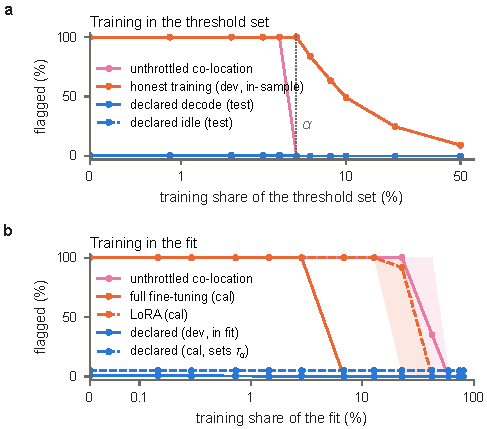
\includegraphics[width=\columnwidth]{f9_contamination.pdf}
  \caption{Training in the reference blinds $s_R$. (a) Honest-training windows added to the threshold set, with the
    fit unchanged and $\alpha = \AlphaPct\%$. The unthrottled run drops to zero near a
    training share of $\alpha$. Honest training is in-sample, since the added windows
    come from its pool. Test decode and idle are flagged less as $\tau_\alpha$ rises.
    (b) Honest-training windows added to the fit, with the threshold set unchanged:
    median over \EfourNDraws{} draws, band from the lowest to the highest draw. Full
    fine-tuning and LoRA are calibration-day runs, outside every fit. The development
    declared windows are in every fit (in-sample). The calibration declared windows set
    $\tau_\alpha$, so their rate stays near $\alpha$ by construction.}
  \label{f:f9}
\end{figure}

The reference is where the signature check can be attacked by an adversarial operator. It is recorded on the
operator's chips, so an operator can try to corrupt it, and even a reference recorded in good
faith can erroneously leave out a declared workload.\footnote{For example, the operator
declares decode, prefill and idle, but the inspectors record only decode. Nobody cheats,
yet the reference is incomplete.} The reference has two parts: the fit, and the threshold set
that fixes $\tau_\alpha$. In \cref{s:works} the fit holds every declared workload, and
the threshold set holds decode and idle.

Here we change the reference in three ways (\cref{f:f10}b--d). Each
change makes the check fail, and each failure is one of two kinds. A \emph{loud} failure
raises alarms on declared work, so the verifier sees that the reference is wrong. A
\emph{silent} failure misses hidden training and raises no alarm on declared work, so
the verifier sees nothing.

\textbf{A declared workload missing from both parts: loud} (\cref{f:f10}b,
\cref{t:t7}). Work that is in neither the fit nor the threshold set raises alarms.
Prefill held out of both is one case (\cref{s:declaration}). A decode-only reference,
with decode alone in the threshold set, is another (\cref{f:f8}c). It detects
\TfourMisCoDeclared\% of co-location, but it is also in alarm for \TfourIdleADecode\% of
test-day idle. A monitor that is almost always in alarm on declared idle is useless, but
it fails loudly. Its alarms show the verifier that it is failing.

\textbf{A declared workload in the threshold set only: silent} (\cref{f:f10}c,
\cref{t:t7}). Keep the decode-only fit, and add idle to its threshold set. The threshold set
now holds decode and idle, which is our default. Idle is now in the threshold set
but not in the fit. It scores high
and lifts $\tau_\alpha$ to \TauDecOnlyPooled{} (\cref{f:f8}d; \cref{f:f7} shows the
scores). The monitor then detects \TfourMisCoPooled\% of co-location and misses all
\EpScored{} episodes. It raises no alarm on test-day decode, just as the complete reference
does. We see that this monitor then fails silently; it does not alert on hidden training, and the verifier has no way to know that it is failing. Prefill is also missing from this fit. Accordingly, with decode alone in the threshold set every prefill window is flagged (\cref{t:t7}). However $\tau_\alpha$ now sits above the prefill scores, and so \DecOnlyPrefillPooled\% of prefill windows are flagged. That is, a missing workload raises alarms only if nothing else
has raised the threshold.

A verifier can expose the silent monitor with a positive control. It gives the monitor
work that it knows to be training, and checks that the monitor flags it. The working
monitor flags \RoneHonestFull\% of development honest training. The silent monitor flags
\TfourPosCtrl\% (\cref{f:f8}, right column).

\textbf{Training in the reference: silent} (\cref{f:f10}c--d, \cref{f:f9}). An operator can
also corrupt the reference, by running training while it is recorded. We test this by
adding windows of training that runs alone on the GPU (honest training,
\cref{s:corpus}) to each part of the reference in turn (\cref{a:reference}). In both cases the monitor comes to miss hidden training, and it
raises no alarm on declared work.

\emph{Training in the threshold set raises $\tau_\alpha$} (\cref{f:f10}c). It takes little training. $\tau_\alpha$ is the $(1-\alpha)$ quantile of the
threshold set (\cref{e:tau}), so once training makes up a fraction $\alpha$ of that set,
$\tau_\alpha$ sits among the training scores. At
$\alpha = \AlphaPct\%$, \EthreeKFive{} windows added to the \EthreeCalWindows{}
calibration windows take detection of the unthrottled run to zero (\cref{f:f9}a). The
higher $\tau_\alpha$ flags declared work less, not more, so the failure is silent. A
positive control of honest training does not expose it, because at that share honest
training is still flagged at $\ge \EthreeHonestMin\%$.

\emph{Training in the fit lowers the scores of training} (\cref{f:f10}d). The fit learns
training as if it were declared work. How much training this takes depends on its kind.
With training at \EfourShareHonest\% of the fit, a full fine-tuning run outside the fit
is flagged at \EfourFullCal\%. The unthrottled run holds longer. Its median detection
reaches \EfourGoneDet\% at a share of \EfourShareGone\% (\cref{f:f9}b). The declared
windows of the fit are flagged at \EfourDeclZero\% with a clean fit, and less as training
is added, so again no alarm shows the failure. This last result is in-sample, because we did not
score held-out declared work under these fits.
